\documentclass[tikz,border=2mm]{standalone}
\usepackage{tikz}

\definecolor{red}{rgb}{1,.5,.6}
\definecolor{blue}{rgb}{.5,.5,1}

\begin{document}
	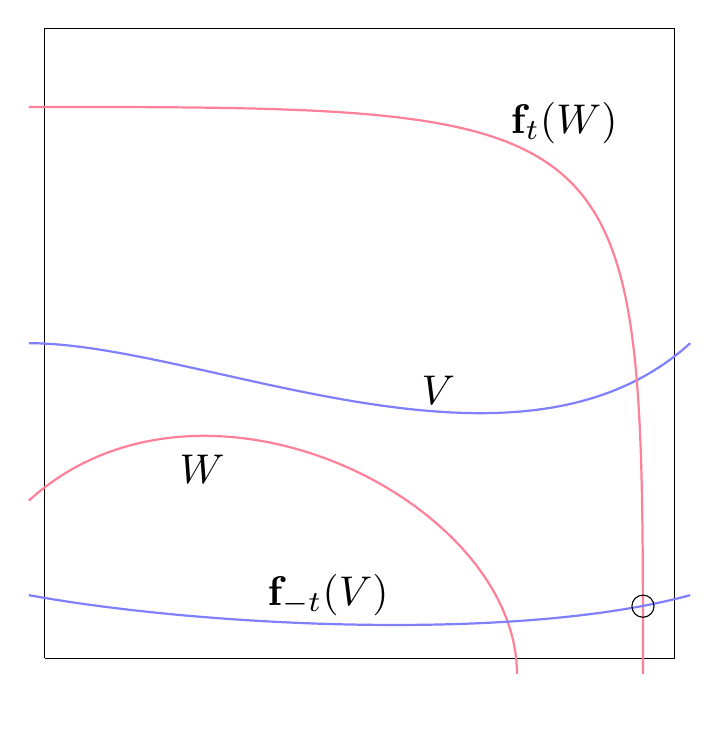
\begin{tikzpicture}[scale = 2]
	
	\draw (0,0) -- (0,4) -- (4,4) -- (4,0) -- (0,0);
	
	\draw[red, thick] (-.1,1) .. controls (1,2) and (3,1).. (3,-.1);
	\draw[blue, thick] (-.1,2) .. controls (1,2) and (3,1).. (4.1,2);
	\draw[red, thick] (-.1,3.5) .. controls (3.8,3.5) .. (3.8,-.1);
	\draw[blue, thick] (-.1,.4) .. controls (1,.2) and (3,.1).. (4.1,.4);
	
	\node[scale=1.5] at (1, 1.2) {$W$};
	\node[scale=1.5] at (2.5, 1.7) {$V$};
	\node[scale=1.5] at (3.3, 3.4) {$\mathbf f_t(W)$};
	\node[scale=1.5] at (1.8, .4) {$\mathbf f_{-t}(V)$};
	
	\node[circle, draw=black, inner sep=0pt, minimum size=8pt] at (3.8,.33) {};
	
	\node[scale=1.5] at (0, -.19) {};
	\end{tikzpicture}
\end{document}